% !TEX encoding = UTF-8 Unicode

\documentclass[a4paper]{article}

%paketi idu ovde
\usepackage{color}
\usepackage{url}
\usepackage[T2A]{fontenc} % enable Cyrillic fonts
\usepackage[utf8]{inputenc} % make weird characters work
\usepackage{graphicx}
\usepackage[english,serbian]{babel}
\usepackage[unicode]{hyperref}
\hypersetup{colorlinks,citecolor=green,filecolor=green,linkcolor=blue,urlcolor=blue}



\begin{document}


\title{Zavisnost od pametnih telefona i njihov uticaj\\
	\small{Seminarski rad u okviru kursa \\
	       Računarstvo i društvo \\
	       Matematički fakultet }
	  }
\author{Luka Miletić \\ mi17091@alas.matf.bg.ac.rs}
\date{1.~decembar 2022.}
\maketitle

\abstract
Broj korisnika pametnih telefona (smartfona, engl. smartphone) širom sveta danas premašuje tri milijarde
i predviđa se dalji rast od nekoliko stotina miliona u narednih nekoliko godina.Razvoj multifunkcionalnih
pametnih telefona i njihova primena promenili su način komuniciranja i informisanja, ali i doveli do
zabrinutosti zbog njihove prekomerne upotrebe i zavisnosti.Poslednjih godina, istraživanja zavisnosti od
pametnih telefona su u porastu. Paralele između prekomerne upotrebe pametnih telefona
i bihevioralne\footnote{Psihološka škola, nastala početkom 20. veka,
koja se bavi istraživanjem objektivnog
ponašanja i načinom rada ljudi;
svoja saznanja crpi iz tačnog posmatranja kako se, pod raznim uslovima, vladaju 
ljudi, osobito deca, i na osnovu tih opažanja, objašnjava duševne procese.}
zavisnosti česte su u israživanjima.
Ovakve stvari nas dovode do činjenice da je „zavisnost od pametnih
telefona” kompleksan fenomen koji zahteva dodatna istraživanja.

\newpage
\tableofcontents
\newpage

\section{Uvod}
Prvo ćemo predstaviti neke, društvu već i poznate, opšte 
karakteristike pametnih telefona u vidu njihovih pozitivnih i negativnih strana
kako bi uveli čitaoce u značaj samog istraživanja uticaja mobilnih telefona
na čoveka i njegovo mentalno tj. fizičko zdravlje.
\newline
Ovaj pregled takodje unapređuje postojeću literaturu o odnosima između
problematične upotrebe pametnih telefona (PSU - problematic smartphone use), 
psihopatologije, zavisničke ličnosti i onlajn društvenog angažmana mladih i odraslih, 
obraćajući pažnju na ponašanja zavisnosti u korišćenju pametnog telefona.
\newline
\newline
U sledećem radu kumuliramo prethodna istraživanja o psihologiji zavisničkog
ponašanja pametnih telefona u smislu problematične upotrebe,
socijalne anksioznosti i depresivnog stresa fokusirajući se na odnos između
upotrebe mobilnih društvenih medija, rizika od zavisnosti od pametnih telefona,
problema mentalnog zdravlja i individualnog blagostanja.
Provereni prikupljeni nalazi dokazuju da depresija i socijalna anksioznost
predstavljaju determinante rizika za veći PSU i da su određene kategorije
aplikacija za pametne telefone pozitivno povezane sa blagostanjem.
\newline
\newline
Buduća uputstva bi trebalo da razjasne da li
kompulsivna upotreba pametnog telefona dugoročno negativno utiče na mentalno
i fizičko zdravlje.
\newline
\newline
Problematična upotreba pametnog telefona (PSU) je složen
fenomen koji se sastoji od različitih disfunkcionalnih
manifestacija (npr. socijalna izolacija, smanjeno samopouzdanje,
depresija i anksioznost) bez potencijalne zavisnosti od ponašanja \cite{phone}.
Pametni telefoni mogu imati negativne posledice na ljudski mozak i povezane
psihološke procese.
Na osnovu psihijatrijskih simptoma, identifikovane su različite
vrste poremećaja korišćenja pametnih telefona, od kojih su neki povezani
sa internet komunikacijom, posebno pošto je PSU povezan sa depresijom
i samopoštovanjem \cite{miss}.
\newline
Pregled takodje pruža dokaze da je PSU negativno povezan sa različitim
pojmovima blagostanja i da su simptomi psihopatologije povezani sa
ozbiljnošću PSU-a, uz slabe dokaze da upotreba pametnog
telefona može izazvati zavisnost kao i poremećaji upotrebe droga i alkohola.


\newpage
\section{Pozitivne strane pametnih telefona}

\subsection{Komunikacija}
Prva pozitivna strana mobilnih telefona je komunikacija. Sa mobilnim telefonima
možete komunicirati sa bilo kim sa bilo kog mesta u bilo koje vreme.
Danas, pametni telefoni koji dolaze su male veličine sto ih čini veoma lakim za
nošenje.Ne morate da sedite pored prijeminka jer vaš mobilni telefon nije
povezan ni sa čim.

\subsection{Zabava}
Mobilni telefoni su postali izvor neograničene zabave.
Stvari za koje nikada nismo mislili da će biti prisutne u mobilnom telefonu
sada su moguće. Pojavili su se pametni telefoni koji ne samo da vam pomažu
u upućivanju poziva, već vam pomažu i da se zabavljate omogućavajući
vam da igrate igrice, slušate muziku i radite mnogo drugih stvari.

\subsection{Beneficije u učenju(studiranju)}
Ako koristite pametni telefon, možete ga iskoristiti u svojim studijama ili poslu.
Pametni telefoni koji dolaze sa operativnim sistemom Android, Apple iOS i Windows
dolaze sa obrazovnim aplikacijama koje se mogu koristiti dok ste na fakultetu.
Ako se bavite poslom, možete instalirati aplikacije
poput skajpa (engl. Skype) koje će vam pomoći u komunikaciji sa klijentima u
pokretu.


\begin{figure}[h!]
\centering
\begin{center}
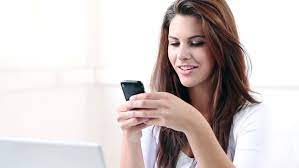
\includegraphics[width=100mm]{image1.jpeg}
\end{center}
\caption{Konzumiranje telefona - komunikacija, zabava}
\label{fig:vr}
\end{figure}


\newpage

\section{Negativne strane pametnih telefona}

\subsection{Zdravstveni problem i incidenti}
Mobilni telefoni dovode do mnogih nesreća.
Mnogi ljudi rade svoj svakodnevni posao, voze dok uzimaju mobilne telefone.
Postoji veliki rizik od nesreće ako razgovarate mobilnim telefonom i vozite
dok pola pažnje posvećujete mobilnom pozivu, a pola pažnje posvećujete putu.

\subsection{Loš uticaj na učenje(studiranje)}
Istina je da mobilni telefoni mogu pomoći studentima u učenju,
ali samo ako ih pametno koriste.
Većina učenika postaje dodatak mobilnim telefonima
i zatekne ih kako igraju igrice, ćaskaju sa prijateljima i gledaju filmove
i druge stvari. Ako su studenti zauzeti da stalno drže pogled na svojim
mobilnim telefonima, neće imati vremena za učenje što bi dovelo do loših ocena.

\begin{verbatim}
\end{verbatim}
\begin{figure}[h!]
\centering
\begin{center}
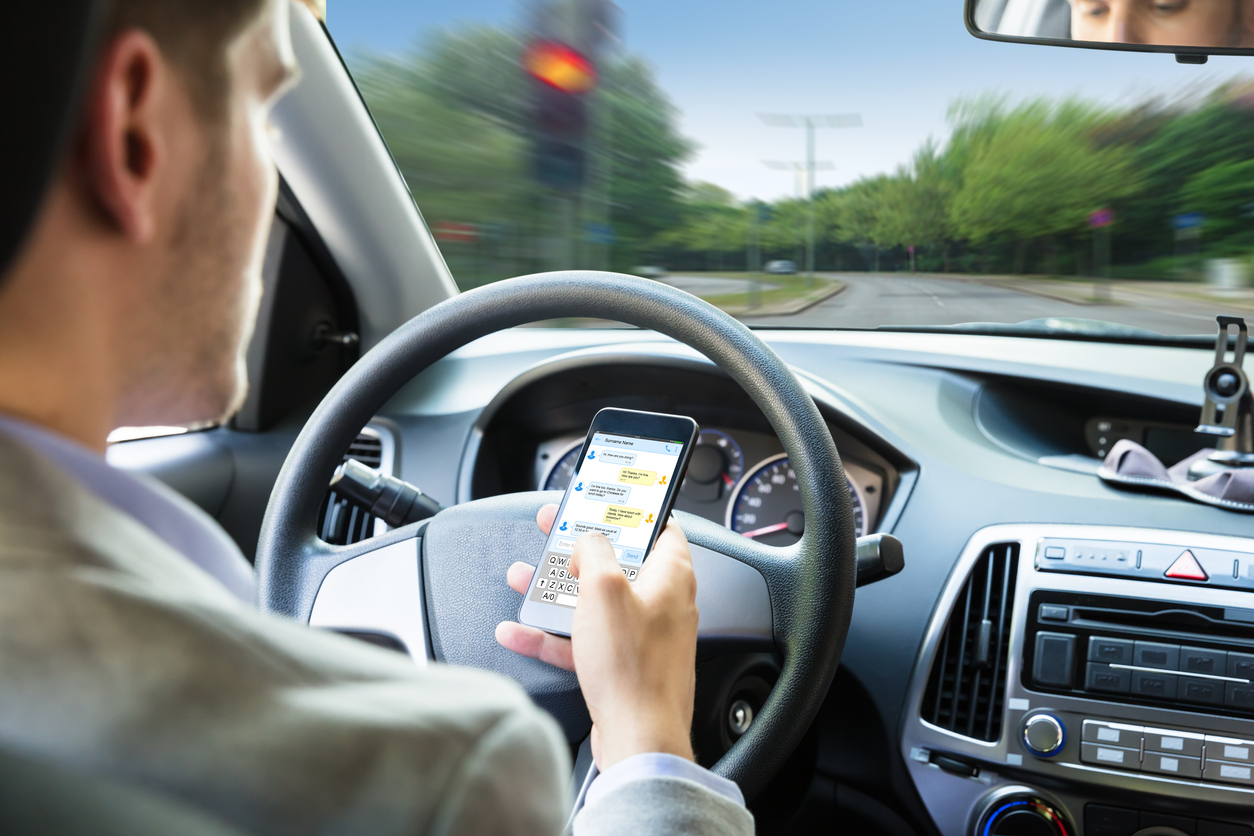
\includegraphics[width=100mm]{image2.jpg}
\end{center}
\caption{Konzumiranje telefona - vožnja}
\label{fig:vr}
\end{figure}


\newpage
\section{Ponašanje zavisnih osoba i fizičko zdravlje}

Fizički negativni efekti su ukorenjeni u prekomernoj upotrebi
pametnih telefona\cite{consume}. Međutim, preterano korišćenje pametnih telefona
može ličiti na zavisnost u smislu neumerene upotrebe,
problema sa kontrolom impulsa i štetnih efekata,
a da nije poremećaj sa ozbiljnim posledicama po fizičko
i psihičko zdravlje \cite{addiction}. Na primer, slanje poruka na
pametnom telefonu je povezano sa napetijim
položajem kičme za razliku od kucanja na računaru.
Uporno savijanje vrata pri korišćenju pametnog telefona predstavlja odrednicu
nelagodnosti u vratu i modifikaciju performansi mišića vrata.
Lepljenje ramena smanjuje bol u vratu bez uticaja na performanse
mišića vrata i umor tokom slanja SMS-ova sa pametnog telefona\cite{addiction}.


Prekomerna upotreba pametnog telefona takođe generiše loše ishode mentalnog
zdravlja, npr. simptomi depresije i problemi sa spavanjem.
Što se tiče usvajanja pametnih telefona i društvenih platformi,
pozitivni rezultati su povezani sa društvenim kapitalom i uključenošću\cite{consume},
dok se štetne posledice razvijaju iz prekomerne upotrebe 
i anksioznosti da budemo stalno aktivni.
Ilustracije radi, nekorišćenje pametnih telefona u spavaćoj sobi
povećava životni standard, a rizik od prekomerne upotrebe pametnog
telefona se smanjuje kada se takvi uređaji drže izvan spavaće sobe.
Spavanje bez pametnih telefona poboljšava kvalitet sna, odnose, motivaciju
i dobro fizičko stanje.
PSU može dovesti do problema sa mobilnošću zglobova, prstiju i vrata.
Za tinejdžere, kvalitet sna utiče na rast,
emocionalnu postojanost i sposobnosti učenja, pa je stoga upotreba
pametnih telefona presudno za adekvatne navike spavanja\cite{consume}.


Osobe koje traže veće senzacije mogu biti posebno izložene riziku od PSU.
Pametni telefoni mogu omogućiti pojedincima da budu uključeni u niz poduhvata
i pomognu im u ublažavanju dosade u slobodno vreme.
Značajniji nivoi dosade u slobodno vreme i traženja senzacija\cite{ethics}
imaju pozitivnu vezu sa višim stepenom prekomerne upotrebe pametnog telefona.
Pametni telefoni mogu izazvati zavisnost,
a njihovi korisnici koji žele da ostvare različite svrhe mogu postati
izuzetno zavisni od njih.
Pojedinci koji imaju jače i jednostavnije osnove da pokušaju da postignu ciljeve
na svojim pametnim telefonima su skloniji da imaju značajniji
nivo prekomerne upotrebe pametnih telefona\cite{factors}.


Prekomerna upotreba pametnog telefona može dovesti do zavisnosti
od telefona koje dalje dovodi do fizičkih i psiholoških
negativnih efekata, utičući, između ostalog, na performanse mišića vrata
i kvalitet sna.



\newpage
\section{Upotreba telefona i društvena ankcioznost}
Postoji umerena veza između upotrebe pametnog telefona i stresa i anksioznosti,
ali ozbiljnost depresije i ozbiljnost anksioznosti su značajno povezane
sa prekomernom upotrebom pametnog telefona \cite{anxiety}.
\newline
Anksioznost i motivacija stanja predstavljaju značajne prediktore PSU.
Objedinjujući različite funkcije, pametni telefoni pružaju tinejdžerima više
mogućnosti za zabavu kako bi ublažili dosadu u slobodno vreme.
Usvajanje pametnih telefona i za međuljudsko umrežavanje i za opuštanje
ima važne i direktne posledice na prekomernu upotrebu pametnih telefona \cite{face},
dok na pojedince koji koriste pametne telefone za praćenje vesti ne utiče PSU.
Nesposobnost da se reguliše zavisnost, bekstvo, anksioznost i
gubitak produktivnosti predstavljaju niz efekata
ponašanja korisnika pametnih telefona koji spadaju u grupu ljudi sa PSU-om.
Značajno otuđenje može eskalirati PSU \cite{addict}.
\newline
Konkretno, nezadovoljstvo imidžom tela je pozitivan prediktor PSU.
Socijalna anksioznost je relevantan posrednik između nezadovoljstva
imidžom tela i PSU. Pored toga, za socijalno anksiozne osobe,
mrežno umrežavanje zasnovano na pametnim telefonima manje opterećuje
živce nego van mreže.
Emocionalno traumatska iskustva su povezana sa PSU
kod tinejdžera i ova veza se može donekle razjasniti nezadovoljstvom
imidžom tela i determinantama psihosocijalnog rizika \cite{child}.
\newline
\newline
Depresija i socijalna anksioznost su korelati PSU.
Psihopatološki simptomi, interpersonalna osetljivost i upotreba
pametnog telefona artikulišu dinamiku ponašanja težine simptoma
socijalne anksioznosti.

\newpage

\section{Zanimljivosti}

Od januara 2016. godine, čak 90 odsto odraslih osoba
u SAD-u posedovalo je mobilni telefon,
a među osobama starim od 18 do 29 godina, 
brojka se dizala na 98 odsto. 
Većina mlađih korisnika koristi pametne telefone,
a ono što je još zanimljivije jeste da mobitele telefone pretežno koristimo
kao društvo.

Evo nekih od najzanimljivih podataka iz SAD-a iz 2016. godine:

\begin{center}
    \begin{tabular}{ |l|l|} 
    \hline
  Vrsta radnje&Vrednost\\
  \hline
  Koristi telefon u toaletu & 61\% \\
  Čita poruke u toaletu & 49\%   \\
  Javlja se na telefon u toaletu & 30\% \\
  Ispustilo telefon u wc šolju & 9\%  \\
  Proveravanje mail-a na telefonu & 78\% \\
  Otvoreno svih mail-ova na telefonu & 53\% \\
  Sluša muziku na telefonu & 48\% \\
  Mladjih osoba koje koriste mobilni za poruke & 97\%(dnevno 87.7 poruka) \\
  \hline  
   
    \hline
    \end{tabular}
\end{center}

Ovi podaci danas se najverovatnije drastično razlikuju i pokazuju neverovatne
brojke jer su mobilni telefoni postali neizostavni deo ljudskog života.

\section{Zaključak}

\textit{Značajna istraživanja su nedavno razmatrala psihologiju zavisničkog
ponašanja pametnih telefona u smislu problematične upotrebe,
socijalne anksioznosti i depresivnog stresa.
Ovaj rad proširuje prethodni rad fokusirajući se na odnos između
upotrebe mobilnih društvenih medija, rizika od zavisnosti od pametnih telefona,
problema mentalnog zdravlja i individualnog blagostanja.
Progresivno relevantni stepeni posedovanja i korišćenja pametnih telefona dovode
do implicitnog rizika od ponašanja zavisnosti i štetnih zdravstvenih rezultata,
oblikujući subjektivno i psihološko blagostanje. Zaključci koji su izvedeni
iz gornjih analiza su da su simptomi depresije i anksioznosti povezani sa
ozbiljnošću PSU-a, generišući, između ostalog, poremećaj emocionalne regulacije,
psihološki stres, loš kvalitet sna i smanjene akademske rezultate.
Osobine ličnosti, socijalno-emocionalni stres i trajanje svakodnevnog
korišćenja pametnog telefona predstavljaju prethodnike PSU-a,
utičući na subjektivno i psihološko blagostanje. Kao ograničenja u ovom pregledu,
ovi rezultati ukazuju na relevantne puteve istraživanja društvenih posledica
zavisnosti mladih odraslih o pametnim telefonima. Buduća uputstva bi trebalo
da razjasne da li kompulzivna upotreba pametnog telefona dugoročno negativno
utiče i na mentalno i na fizičko zdravlje.}




\newpage
\addcontentsline{toc}{section}{Literatura}
\appendix

\iffalse
\bibliography{seminarski} 
\bibliographystyle{plain}
\fi

\begin{thebibliography}{10}

\bibitem{phone} Pivetta E, Harkin L, Billieux J, Kanjo E, Kuss DJ. 
Problematic smartphone use: An empirically validated model.
Comput Hum Behav (2019) 100:105–17. doi: 10.1016/j.chb.2019.06.013

\bibitem{miss} Bratu S. Fear of missing out, improper behavior,
and distressing patterns of use. An empirical investigation.
Linguist Philos Invest (2018) 17:130–40. doi: 10.22381/LPI1720187

\bibitem{anxiety} Elhai JD, Dvorak RD, Levine JC, Hall BJ.
Problematic smartphone use: A conceptual overview and systematic review
of relations with anxiety and depression psychopathology.
J Affect Disord (2017) 207:251–9. doi: 10.1016/j.jad.2016.08.030

\bibitem{face}  Burwell C, Lăzăroiu G, Rothchild N, Shackelford V.
Social networking site use and depressive symptoms:
Does Facebook activity lead to adverse psychological health?
Linguist Philos Invest (2018) 17:141–58. doi: 10.22381/LPI1720188

\bibitem{addict} Lian L. Alienation as Mediator and 
Moderator of the Relationship between Virtues and Smartphone Addiction among
Chinese University Students. Int J Ment Health Addict (2018) 16:1208–18. doi: 10.1007/s11469-017-9842-z

\bibitem{child}  Emirtekin E, Balta S, Sural İ., Kircaburun K,
Griffiths MD, Billieux J.
The role of childhood emotional maltreatment and body image dissatisfaction
in problematic smartphone use among adolescents.
Psychiatry Res (2019) 271:634–9. doi: 10.1016/j.psychres.2018.12.059

\bibitem{addiction} Panova T, Carbonell X.
Is smartphone addiction really an addiction? J Behav Addict (2018)
7:252–9. doi: 10.1016/j.apergo.2017.10.018

\bibitem{consume}  Mirică (Dumitrescu) C-O.
The behavioral economics of decision making: Explaining consumer
choice in terms of neural events.
Econ Manage Financ Mark (2019) 14(1):16–20. doi: 10.22381/EMFM14120192

\bibitem{ethics} Mircică N. The ethics of envy on Facebook.
Anal Metaphys (2017) 16:124–30. doi: 10.22381/AM1620178

\bibitem{factors} Jiang Q, Li Y. Factors affecting
smartphone dependency among the young in China.
Asian J Commun (2018) 28:508–25. doi: 10.1080/01292986.2018.1431296
 
\end{thebibliography}	

\end{document}
